\documentclass[letterpaper]{article}

\usepackage{cite}
\usepackage[utf8]{inputenc}
\usepackage{graphicx}
\usepackage{hyperref}
\usepackage{amsmath,amsthm,amssymb,mathtools}
\usepackage{prftree}

\usepackage{tikz}
\usetikzlibrary{calc,positioning,fit,shapes}

\newcommand{\todo}[1]{{\color{red}[TODO: #1]}}

% notation
\newcommand{\utv}{\alpha}             % universal type variable
\newcommand{\etv}{\widehat{\beta}}    % existential type variable

\title{The Parsley Data Definition Language}
\author{The Parsley Team}

\begin{document}
\maketitle

\begin{abstract}
  Any program that reads formatted input relies on parsing software to
  check the input for validity and transform it into a representation
  suitable for further processing.  Many security vulnerabilities can
  be attributed to poorly defined grammars, incorrect parsing, and
  sloppy input validation.  In contrast to the syntax for programming
  languages, grammars for even common data formats such as DNS and PDF
  are typically context-sensitive and heterogenous.  However, as in
  programming languages, a standard notation or {\em language} to
  express these data format grammars can address poor or ambiguous
  definitions, and the automated generation of correct-by-construction
  parsers from such grammar specifications can yield correct and type-
  and memory-safe data parsing routines.

  This document describes the design of Parsley, a declarative data
  format definition language that combines grammars and constraints in
  a modular way.  It describes the syntax, type system and semantics
  of the language.  It will eventually describe its compiler, which
  will generate an executable parsing library from a Parsley
  specification, and other outputs to enable the verification of the
  correctness of generated parser.
\end{abstract}

\section{Language Design}
\label{s:design}

The language has the following design goals:

\begin{itemize}
\item A useful foundational set of parser primitives and combinators,
\item A capacity to capture context-sensitivity and data-dependency
  via a constraint system, and
\item  A module system that enables nested grammars and composes with
  the constraint system.
\end{itemize}

We employ the following techniques to achieve these goals:

\begin{itemize}
\item The core structure of a Parsley specification is provided by a
  {\em parsing expression grammar (PEG)} \cite{ford2004popl},
  specified in notation similar to {\em extended BNF (EBNF)} for
  grammar productions.  Although {\em context-free grammars (CFGs)}
  use the EBNF notation, there are critical differences in the PEG
  notation: (a) the choice combinator in PEGs is ordered, as opposed
  to non-deterministic in CFGs, and (b) the PEG notation includes
  syntactic predicates that do not occur in CFGs.  The choice of a PEG
  core provides us a core set of primitives and combinators we can
  build on.

\item Context management is provided by a fairly traditional
  attribute-grammar system, where the expression language for
  attribute computations is purely functional and strongly-typed.  In
  Parsley, non-terminals have user-defined attributes, while terminals
  have a default attribute value of type byte or byte-string.  This
  provides us with the tools needed to capture context-sensitivity.

\item Additional context-sensitivity is provided by a constraint
  system that guards further processing within a non-terminal
  production.  The constraint language uses the attribute system to
  perform context-sensitive checks, and cleanly enables data-dependent
  parsing.

\item A module system allows the composition of independent grammars.
\end{itemize}

The expression sublanguage used in attribute updates and constraints
is a strongly typed polymorphic functional language supporting
user-defined types and functions.  It includes a standard library of
common types and utility functions.  The expression and data type
sublanguage is designed to ensure that recursive and iterative
computations always terminate.

\section{Language Use}
\label{s:use}

\begin{figure*}[!ht]
  \centering
  \resizebox{10cm}{!}{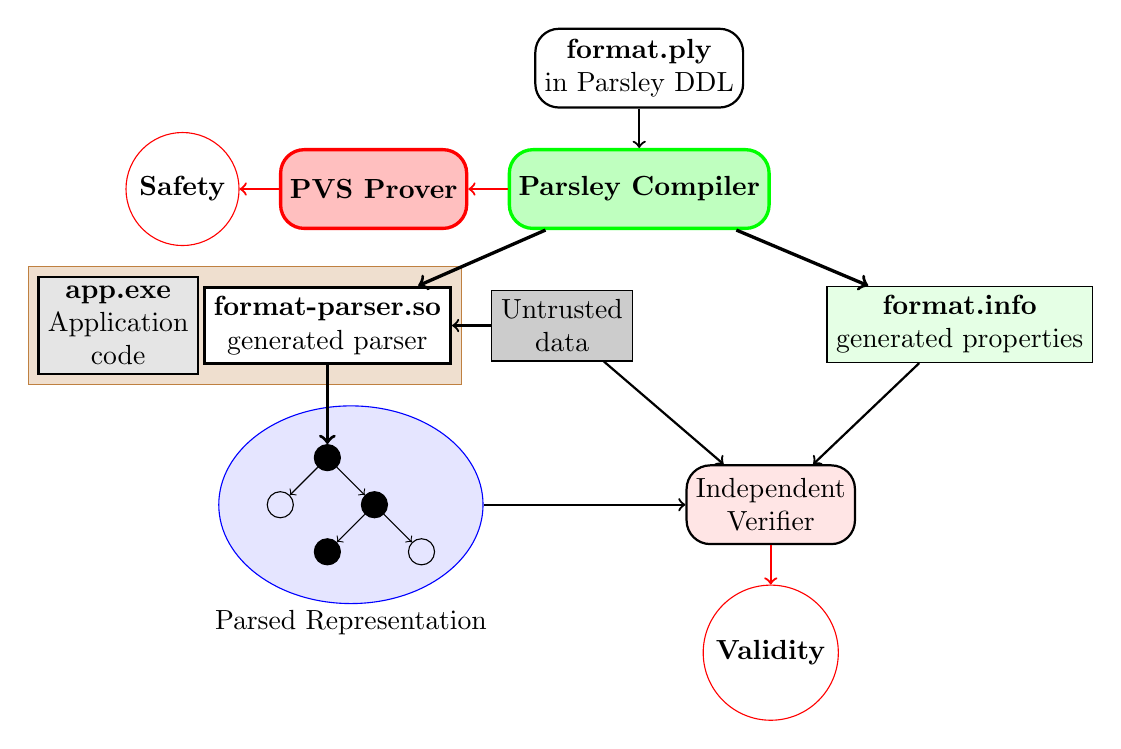
\begin{tikzpicture}[
    node distance=5mm,
    align=center,
    spec/.style={rectangle, rounded corners=3mm, minimum size=10mm, draw=black, thick},
    info/.style={rectangle, draw=black, fill=green!10!white},
    lib/.style={rectangle, very thick, draw=black, fill=white},
    app/.style={rectangle, thick, draw=black, fill=black!10!white},
    prog/.style={rectangle, draw=brown, fill=brown!25!white},
    compiler/.style={rectangle, rounded corners=3mm, minimum size=10mm,
      very thick, draw=green, fill=green!25!white},
    prover/.style={rectangle, rounded corners=3mm, minimum size=10mm,
      very thick, draw=red, fill=red!25!white},
    verifier/.style={rectangle, rounded corners=3mm, minimum size=10mm,
      thick, draw=black, fill=red!10!white},
    data/.style={rectangle, draw=black, fill=black!20!white},
    prop/.style={circle, draw=red},
    ast/.style={circle, draw=black},
    memory/.style={ellipse, draw=blue, fill=blue!10!white},
    input/.style={->, thick, black},
    gen/.style={->, very thick, black},
    proverinput/.style={->, thick, red},
    proveroutput/.style={->, thick, red},
    tree/.style={->, black},
  ]

  \pgfdeclarelayer{background}
  \pgfdeclarelayer{main}
  \pgfdeclarelayer{foreground}
  \pgfsetlayers{background,main,foreground}

  % main pipeline
  \begin{pgfonlayer}{main}
    \node (spec)      [spec]                         {\textbf{format.ply}\\ in Parsley DDL};

    \node (compiler)  [compiler, below=of spec]      {\textbf{Parsley Compiler}};

    \node (prover)    [prover, left=of compiler]     {\textbf{PVS Prover}};

    \node (safety)    [prop,left=of prover]          {\textbf{Safety}};

    \node (lib)       [lib, below left=1cm of compiler]   {\textbf{format-parser.so}\\ generated parser};

    \node (info)      [info, below right=1cm of compiler] {\textbf{format.info}\\ generated properties};

    \node (app)       [app, left=0.5mm of lib]       {\textbf{app.exe}\\ Application\\ code};

    \node (data)      [data, right=of lib]           {Untrusted\\ data};
  \end{pgfonlayer}

  % complete application
  \begin{pgfonlayer}{background}
    \node (prog)      [prog, fit=(app.south west) (app.north west)
                                 (lib.south east) (lib.north east)] {};
  \end{pgfonlayer}

  % generated AST in memory
  \begin{pgfonlayer}{main}
    \node (root)      [ast, fill=black, below] at ($(lib.south)+(0,-1cm)$)  {};

    \node (c0)        [ast, below left=of root] {};
    \node (c1)        [ast, below right=of root, fill=black] {};
    \node (c10)       [ast, below left=of c1, fill=black] {};
    \node (c11)       [ast, below right=of c1] {};
  \end{pgfonlayer}
  \begin{pgfonlayer}{background}
    \node (tree)      [memory, fit=(root) (c0) (c1) (c10) (c11)] {};
  \end{pgfonlayer}

  \begin{pgfonlayer}{main}
    \node (appdata)   [below=-0.5mm of tree] {Parsed Representation};
    \node (verifier)  [verifier] at (compiler.south east |- tree) {Independent\\Verifier};
    \node (validity)  [prop, below=of verifier] {\textbf{Validity}};
  \end{pgfonlayer}

  % flow
  \draw[input]         (spec) -- (compiler);
  \draw[gen]           (compiler) -- (lib);
  \draw[gen]           (compiler) -- (info);
  \draw[proverinput]   (compiler) -- (prover);
  \draw[proveroutput]  (prover) -- (safety);

  \draw[input]         (data) -- (lib);

  \draw[gen]           (lib) -- (root);
  \draw[tree]          (root) -- (c0);
  \draw[tree]          (root) -- (c1);
  \draw[tree]          (c1) -- (c10);
  \draw[tree]          (c1) -- (c11);

  \draw[input]         (tree) -- (verifier);
  \draw[input]         (info) -- (verifier);
  \draw[input]         (data) -- (verifier);
  \draw[proveroutput]  (verifier) -- (validity);

\end{tikzpicture}
}
  \caption{Parsley in context.}
  \label{f:pipeline}
\end{figure*}

The typical use of a Parsley specification is via the workflow
illustrated in Figure~\ref{f:pipeline}.

The Parsley compiler performs type and semantic checks on a given
Parsley specification.  The type checks correspond to standard
polymorphic type checking~\cite{Dunfield13:bidir}\cite{zhao19:bidir},
with rules to handle grammar productions.  In addition, attribute
usage checks are performed, such as for $L$-attributedness (see
below).

The compiler generates prover definitions that are used to perform
safety checks: for example, a check to ensure that data-dependent
constructs do not use a data value as an array index without an
appropriate constraint check.  We are developing the safety properties
that can be used by the PVS theorem prover to verify that the Parsley
specification is a `safe' grammar.

We are also defining the parsing automaton that will be generated by
the compiler.  This automaton needs to interleave constraint and
attribute computation with parsing actions that construct the internal
data representation and manipulate the parsing buffer.  When used for
efficiently parsing data, especially network protocols, attribute
computations have to be done on partially constructed parse trees
(unlike the typical use of attribute grammars in programming
languages, where the entire parse tree of a program can be available
before processing).  In our experience of using Parsley to define data
formats, the computations in constraints and attribute updates require
access to a parsing context (via inherited attributes) that is best
handled by $L$-attributed grammars, which are compatible with the
top-down processing of the ``core'' PEG specification.  $L$-attributed
grammars are attribute grammars where attributes in the nodes in the
parse tree to the left of the current node have been assigned their
final values.  This eases the implementation of PEG backtracking, as
assigned attribute values do not need to be unwound.  The generated
automaton is compiled into a library that can be linked into
application code.  We plan to use a Rust code generator to ensure that
the library is type and memory safe, can be linked into C
applications, and is compatible with other languages using the
appropriate wrappers.

The data representation constructed by the automaton contains a {\em
  proof of parse}.  We are building on the approach used in
~\cite{Blaudeau_2020}, which formalized PEG parsing and the generation
of verifiable PEG parsers.  These parsers annotate the constructed
data representation with grammar metadata that can be used to verify
that the representation is a valid parse of the given input data for
the given Parsley specification.  This verification is done in an
independent verifier, which is simple enough to include in the
application itself.

\subsection*{Unresolved issues}

The API between the application and the parsing library will dictate
crucial implementation choices, and hence impact the code generation
pipeline.  This API might differ across applications parsing the same
format, and these types of API often differ across different types of
formats (e.g. streaming network formats versus document formats).

A crucial requirement is to ensure that the parsing automaton is not
Turing-complete; i.e. arbitrary input data cannot cause
Turing-complete computation within the parsing library.  We are
attempting to provide formal guarantees that this will be the case.

\section{Abstract syntax}
\label{s:syntax}

The abstract syntax of Parsley is shown in
Figure~\ref{f:parsley-syntax}, and has two layers: the expression
sublanguage is shown first, followed by the grammar sublanguage.

\begin{figure}
  \begin{tabular}{l c l l}
    Paths        & $p$      & ::= & $ x \mid p.x $ \\
    Constants    & c        & ::= & 0,1,\ldots\ $|$\ `A', `B', \ldots\ $|$\ \ldots \\
    Constructors & C        &     & \\
    Attributes   & $l$      & ::= & $ l^i \mid l^s $ \\
    Base types   & $\nu$    & ::= & $ \texttt{unit} \mid \texttt{uint8} \mid \texttt{int32} \mid \ldots $ \\
    Monotypes    & $\tau$   & ::= & $ \utv \mid \nu \mid (\tau_i) \mid \tau\rightarrow\tau \mid \sum_i C_i\tau_i \mid \{l_i:\tau_i\} \mid \texttt{typeof}(N) $ \\
    Types        & $\sigma$ & ::= & $ \tau \mid \forall\utv.\sigma \mid \sigma\rightarrow\sigma $ \\
    Expressions  & $e$      & ::= & $ p \mid \textrm{c} \mid C e \mid (e_i) \mid e\ e \mid e\ \texttt{op}\ e \mid (e : \tau) \mid e.l $ \\
                 &          &     & $\mid \textrm{case }e\ \{\rho_i, e_i\} \mid \textrm{let }x=e\textrm{ in }e \mid e \sim C \mid f\ e $ \\
    Patterns     & $\rho$   & ::= & $ x \mid (\rho_i) \mid C\rho $ \\
    Functions    & $f$      & ::= & $ x := (x_i:\sigma_i)\rightarrow\sigma \{e\} $ \\
    Statements   & $s$      & ::= & $ p = e $ \\
                 &          &     & \\
    Constraints  & $\phi$   & ::= & $ e $ \\
    Actions      & $a$      & ::= & $ \{s_i\} $ \\
    Rules        & $r$      & ::= & $ \epsilon \mid \textrm{c} \mid (x=)^?N\{l_i=e_i\} \mid \phi r $ \\
                 &          &     & $\mid r r \mid r / r \mid r^{*e?} \mid !r \mid !^Rr \mid a $ \\
    Productions  & $P$      & ::= & $ N\{l_i:\tau_i\} := r $ \\
    Format       & $F$      & ::= & $ \{ \tau_i, N\{l_i:\tau_i\}, P_i \} $ \\
  \end{tabular}
  \caption{Abstract syntax of the Parsley specification language}
  \label{f:parsley-syntax}
\end{figure}

\subsection*{Expression sublanguage}
\label{ss:lang:expr}

In Figure~\ref{f:parsley-syntax}, $x$ over identifiers, $l$ over
inherited $l^i$ and synthesized $l^s$ attributes, $\utv$ ranges over
type variables, and $op$ over standard arithmetic and boolean
operators.  Paths $p$ are used to access identifiers across modules.

The type system is a conventional polymorphic type system
with records.  It is equipped with a set of standard base types $\nu$, type
constructors like tuples $(\tau_i)$, functions $\tau\rightarrow\tau$,
sums $\sum_iC_i\tau_i$, records $\{l_i:\tau_i\}$ and
polymorphic type schemes $\forall\utv.\tau$.  The Parsley library
defines standard data types such as polymorphic lists, sets, and maps.

The expression language is also standard, with tuples $(e_i)$, sums
$C_i e_i$, function application $e\ e$, attribute or record field
selection $e.l$, type constraints $(e:\tau)$, and let bindings and
case expressions that bind patterns within expressions.  The
$e\ \sim\ C$ is a boolean expression that tests if $e$ is a sum with
the $C$ constructor; this is a useful primitive within grammar
constraints.

Parsley supports user-defined higher-ranked polymorphic functions $f$,
where the function arguments have polymorphic types.  The supporting
type system is described in \S\ref{s:typesys}.

Statements are the only imperative constructs, and consist of
assignments to (synthesized) attributes.

\subsection*{Grammar sublanguage}
\label{ss:lang:grammar}

We now come to the grammatical constructions: productions, rules, and
actions.  These are based on parsing expression grammars (PEGs)
\cite{ford2004popl}, but are extended with an attribute system and
constraints to capture context sensitivity.  A grammar production
defines the parsing expression for a non-terminal $N$.  Each $N$ is
typed as a record named $\texttt{typeof}(N)$ with its attributes as
the record fields.  Rules $r$ are elemental parsing expressions and
are combined with parsing combinators.  Actions $a$ are used to update
parsing state during parsing, and consist of a sequence of statements
where synthesized attributes are assigned.  The primitive rules are
$\epsilon$, which successfully matches without consuming any input,
and literals $\textrm{c}$, which match if the input has a $c$ prefix,
upon which that prefix is consumed.  The $N\{l_i=e_i\}$ rule matches
if its production matches an input prefix given its inherited
attributes $l_i$ are initialized as specified with expressions $e_i$
evaluated within the parsing context at that point.  The $x=N$
construct names the matched value (of type $\texttt{typeof}(N)$), and
enables access to the values of its attributes as $x.l$ in expressions
appearing within any subsequent constraints, actions, or attribute
initializations.

These primitive rules can be combined with combinators, as in PEG, but
with some extensions.  $r\ r$ denotes the PEG sequence operator, while
$r\ /\ r$ is the PEG ordered choice.  The $!r$ construct is the
\emph{not} syntactic predicate in PEG.  $r^{*e?}$ denotes the Kleene
star, but with an optional bound $e$ that is context sensitive.  If
the bound is present, it limits the number of times that $r$ is
matched.

A parsing rule $r$ can be guarded with a constraint expression $\phi$,
written as $\phi\ r$: the boolean expression $\phi$ is evaluated
before deciding to proceed parsing with rule $r$.  This is a Parsley
extension of PEG, and could be thought of as a \emph{contextual}
predicate: $\phi$ can check the current parsing state, using the
attribute values of syntactic elements in its context.  If this guard
fails, parsing backtracks to the most recent choice point, and
continues with the next alternative.

Parsley is equipped with a module system that enables splitting a
specification into multiple files, and allows data specifications to
be re-used in different contexts.  Paths support the module system
(not shown) by enabling cross-module use of types and syntax elements.

\subsection*{Extensions under development}

The Parsley language is a work-in-progress, and is being adapted as we
attempt to use it to capture more data formats.  The parsing of a PDF
file involves seeking to the end of the file (or a specific marker)
and searching backwards for a syntactic element.  This motivated the
$!^Rr$ construct, which can be considered as a \emph{reverse-not}
predicate: it checks backwards from the current parsing location
whether the parse buffer matches $r$.

We are also considering extending Parsley with primitives to capture
manipulations of the current parsing offset by actions such as
seeking.  Such offset manipulation could either derive declaratively
from the format specification, or procedurally under the control of
the application driving the parser.  A design challenge is to ensure
both types of manipulations are supported and compose well.  In
addition, this is one of the most security-critical aspects of
parsing: ensuring that offsets derived from untrusted data are used in
valid ways.

\section{Type system}
\label{s:typesys}

The polymorphic type system used in Parsley supports higher-ranked
polymorphism with type-inference, using a bidirectional scheme based
on~\cite{Dunfield13:bidir}.  It requires type annotations for
polymorphic function arguments, and allows only predicative type
inference.  This system relies on a polymorphic subtyping scheme
\cite{odersky96} to guide instantiation of polymorphic quantifiers.
We extend this system to the Parsley grammar language as described
below.

Figures~\ref{f:defs:wf:types:worklists} and \ref{f:wf:judgments}
define the algorithmic worklist $\Gamma$, and show the mutually
recursive rules for a well-formed context judgment, $\vdash\Gamma$,
and a well-formed type judgment, $\Gamma\vdash\tau$.  The worklist
$\Gamma$ integrates the traditional binding context and the pending
judgments into a single entity, easing the tracking and management of
variable scoping.  These definitions follow the ordered algorithmic
worklist model of~\cite{zhao2018,zhao19:bidir}, which provides
convenient scoping of type variables introduced during type-checking.
Figure~\ref{f:wf:expressions} defines well-formed expressions.

\begin{figure}
  \begin{tabular}{l c l l l}
    Existential variables & $\etv$   &     &                                   & \\
    Monotypes             & $\tau$   & ::= & $ \utv\ \ldots $                  & as in Figure~\ref{f:parsley-syntax} \\
    Algorithmic types     & $\sigma$ & ::= & $ \etv $                          & \\
                          &          &     & $ \mid \tau\ \ldots $             & as in Figure~\ref{f:parsley-syntax} \\
                          &          &     &                                   & \\
    Judgment chain        & $\omega$ & ::= & $ \sigma_1\leq\sigma_2 $          & subtyping judgment \\
                          &          &     & $ e\Leftarrow\sigma $             & checking judgment \\
                          &          &     & $ e\Rightarrow_\utv\omega $       & inference judgment \\
                          &          &     & $ \sigma\bullet e\rightsquigarrow_\utv\omega $ & application inference judgment \\
                          &          &     &                                   & \\
    Worklist              & $\Gamma$ & ::= & $ \cdot $                         & empty context \\
                          &          &     & $ \mid\Gamma, x: \tau $           & program variable \\
                          &          &     & $ \mid\Gamma, N: \{l_i:\tau_i\} $ & non-terminal \\
                          &          &     & $ \mid\Gamma, \utv $              & universal type variable \\
                          &          &     & $ \mid\Gamma, \etv  $             & existential type variable\\
                          &          &     & $ \mid\Gamma\Vdash\omega $        & work \\

  \end{tabular}
  $$ \boxed{\vdash\Gamma}\ \textrm{Well-formed worklist} $$
  $$ \prftree[r]{$\mathtt{wf_w uvar}$}
             {\prfassumption{\utv\notin\Gamma}}
             {\vdash\Gamma, \utv}\qquad
     \prftree[r]{$\mathtt{wf_w evar}$}
             {\prfassumption{\etv\notin\Gamma}}
             {\vdash\Gamma, \etv}\qquad
     \prftree[r]{$\mathtt{wf_w pvar}$}
             {\prfassumption{x\notin\Gamma}}{\prfassumption{\Gamma\vdash\sigma}}
             {\vdash\Gamma, x:\sigma} $$
  $$ \prftree[r]{$\mathtt{wf_w N}$}
             {\prfassumption{N\notin\Gamma}}{\prfassumption{\Gamma\vdash\{l_i:\tau_i\}}}
             {\vdash\Gamma, N:\{l_i:\tau_i\}}\qquad
     \prftree[r]{$\mathtt{wf_\omega}$}
             {\prfassumption{\vdash\Gamma}}{\prfassumption{\Gamma\vdash\omega}}
             {\vdash\Gamma\Vdash\omega} $$

  $$ \boxed{\Gamma\vdash\sigma}\ \textrm{Well-formed type}  $$
  $$ \prfbyaxiom{$\mathtt{wf_t \nu}$}{\Gamma\vdash\nu}\qquad
     \prftree[r]{$\mathtt{wf_t tvar}$}
             {\prfassumption{\utv\in\Gamma}}
             {\Gamma\vdash\utv}\qquad
     \prftree[r]{$\mathtt{wf_t evar}$}
             {\prfassumption{\etv\in\Gamma}}
             {\Gamma\vdash\etv}\qquad
     \prftree[r]{$\mathtt{wf_t typeof}$}
             {\prfassumption{N\in\Gamma}}
             {\Gamma\vdash\texttt{typeof}(N)} $$
  $$ \prftree[r]{$\mathtt{wf_t \forall}$}
             {\prfassumption{\Gamma,\utv\vdash\sigma}}
             {\Gamma\vdash\forall\utv.\sigma}\qquad
     \prftree[r]{$\mathtt{wf_t \rightarrow}$}
             {\prfassumption{\Gamma\vdash\sigma_1}}{\prfassumption{\Gamma\vdash\sigma_2}}
             {\Gamma\vdash\sigma_1\rightarrow\sigma_2}\qquad
     \prftree[r]{$\mathtt{wf_t tup}$}
             {\prfassumption{\Gamma\vdash\tau_i\ \forall i}}
             {\Gamma\vdash(\tau_i)} $$
  $$ \prftree[r]{$\mathtt{wf_t sum}$}
             {\prfassumption{\forall i,j:C_i=C_j\Rightarrow i=j}}
             {\prfassumption{\Gamma\vdash\tau_i\ \forall i}}
             {\Gamma\vdash\sum_i C_i\tau_i}\qquad
     \prftree[r]{$\mathtt{wf_t rec}$}
             {\prfassumption{\forall i,j:l_i=l_j\Rightarrow i=j}}
             {\prfassumption{\Gamma\vdash\tau_i\ \forall i}}
             {\Gamma\vdash\{l_i:\tau_i\}} $$
  \caption{Well-formed types and worklists}
  \label{f:defs:wf:types:worklists}
\end{figure}

\begin{figure}
  $$ \boxed{\Gamma\vdash\omega}\ \textrm{Well-formed judgment} $$
  $$ \prftree[r]{$\mathtt{wf_\omega \leq}$}
             {\prfassumption{\Gamma\vdash\sigma_1}}{\prfassumption{\Gamma\vdash\sigma_2}}
             {\Gamma\vdash\sigma_1\leq\sigma_2}\qquad
     \prftree[r]{$\mathtt{wf_\omega\Leftarrow}$}
             {\prfassumption{\Gamma\vdash e}}{\prfassumption{\Gamma\vdash\sigma}}
             {\Gamma\vdash e\Leftarrow\sigma}\qquad
     \prftree[r]{$\mathtt{wf_\omega\Rightarrow}$}
             {\prfassumption{\Gamma\vdash e}}{\prfassumption{\Gamma,a\vdash\omega}}
             {\Gamma\vdash e\Rightarrow_\utv\omega} $$
  $$ \prftree[r]{$\mathtt{wf_\rightsquigarrow}$}
             {\prfassumption{\Gamma\vdash\sigma}}{\prfassumption{\Gamma\vdash e}}
             {\prfassumption{\Gamma,a\vdash\omega}}
             {\Gamma\vdash\sigma\bullet e\rightsquigarrow_\utv\omega} $$
  \caption{Well-formed judgments}
  \label{f:wf:judgments}
\end{figure}

\begin{figure}
  $$ \boxed{\Gamma\vdash C}\ \textrm{Well-formed constructors} $$
  $$ \prftree[r]{$\mathtt{wf_C}$}
             {\prfassumption{\sum_i C_i\tau_i\in\Gamma}}{\prfassumption{C\in\{C_i\}}}
             {\Gamma\vdash C} $$
  $$ \boxed{\Gamma\vdash l}\ \textrm{Well-formed labels} $$
  $$ \prftree[r]{$\mathtt{wf_l}$}
             {\prfassumption{\{l_i:\tau_i\}\in\Gamma}}{\prfassumption{l\in\{l_i\}}}
             {\Gamma\vdash l} $$
  $$ \boxed{\Gamma\vdash l}\ \textrm{Well-formed patterns} $$
  $$ \prfbyaxiom{$\mathtt{wf_\rho var}$}
             {\Gamma\vdash x}\qquad
     \prftree[r]{$\mathtt{wf_\rho tup}$}
             {\prfassumption{\Gamma\vdash\rho_i\ \forall i}}
             {\Gamma\vdash (\rho_i)}\qquad
     \prftree[r]{$\mathtt{wf_\rho C}$}
             {\prfassumption{\Gamma\vdash C}}{\prfassumption{\Gamma\vdash\rho}}
             {\Gamma\vdash C\rho} $$
  $$ \boxed{\Gamma\vdash e}\ \textrm{Well-formed expressions} $$
  $$ \prftree[r]{$\mathtt{wf_e pvar}$}
             {\prfassumption{x:\sigma\in\Gamma}}
             {\Gamma\vdash x}\qquad
     \prfbyaxiom{$\mathtt{wf_e \nu}$}
             {\Gamma\vdash \mathrm{c}}\qquad
     \prftree[r]{$\mathtt{wf_e app}$}
             {\prfassumption{\Gamma\vdash e_1}}{\prfassumption{\Gamma\vdash e_2}}
             {\Gamma\vdash e_1\ e_2} $$
  $$ \prftree[r]{$\mathtt{wf_e tup}$}
             {\prfassumption{\Gamma\vdash e_i\ \forall i}}
             {\Gamma\vdash (e_i)}\qquad
     \prftree[r]{$\mathtt{wf_e anno}$}
             {\prfassumption{\Gamma\vdash e}}{\prfassumption{\Gamma\vdash\tau}}
             {\Gamma\vdash (e : \tau)}\qquad
     \prftree[r]{$\mathtt{wf_e op}$}
             {\prfassumption{\Gamma\vdash e_1}}{\prfassumption{\Gamma\vdash e_2}}
             {\Gamma\vdash e_1\ \texttt{op}\ e_2} $$
  $$ \prftree[r]{$\mathtt{wf_e attr}$}
             {\prfassumption{\Gamma\vdash e}}{\prfassumption{\Gamma\vdash l}}
             {\Gamma\vdash e.l}\qquad
     \prftree[r]{$\mathtt{wf_e sum}$}
             {\prfassumption{\Gamma\vdash C}}{\prfassumption{\Gamma\vdash e}}
             {\Gamma\vdash C e}\qquad
     \prftree[r]{$\mathtt{wf_e match}$}
             {\prfassumption{\Gamma\vdash C}}{\prfassumption{\Gamma\vdash e}}
             {\Gamma\vdash e \sim C} $$
  $$ \prftree[r]{$\mathtt{wf_e case}$}
             {\prfassumption{\Gamma\vdash e}}{\prfassumption{\Gamma\vdash\rho_i\ \forall i}}
             {\prfassumption{\Gamma,[\mathrm{bind}(\rho_i)]\vdash e_i\ \forall i}}
             {\Gamma\vdash\textrm{case}\ e\ \{\rho_i, e_i\}} $$
  $$ \prftree[r]{$\mathtt{wf_e let}$}
             {\prfassumption{\Gamma\vdash e_1}}{\prfassumption{\Gamma\vdash\rho}}
             {\prfassumption{\Gamma,[\mathrm{bind}(\rho)]\vdash e_2}}
             {\Gamma\vdash\textrm{let}\ \rho=e_1\ \textrm{in}\ e_2} $$
  \caption{Well-formed expressions}
  \label{f:wf:expressions}
\end{figure}

\todo{adding paths and path resolution.}

Figures~\ref{f:typecheck:std} and ~\ref{f:typecheck:parsley} show the
typing rules for Parsley, deriving again from the worklist approach
of~\cite{zhao2018,zhao19:bidir}.  The main typing rules take the
judgment at the head of the worklist, and either solve it or break it
into smaller judgments that are pushed onto the worklist; this repeats
until the worklist is empty.  In order to solve for unknown types, the
process introduces {\em existential type variables} $\etv$ into the
context, and when such a variable is solved, the solution is
immediately substituted into the worklist before proceeding.

\newcommand\rstep[1]{~\longrightarrow_{\makebox[0pt][l]{$\scriptstyle #1$}\phantom{~~}}}
\newcounter{ruleCounter}
\newcommand\typrule{\stepcounter{ruleCounter}\rstep{\arabic{ruleCounter}}}

\begin{figure}
  $$ \boxed{\Gamma\vdash\Gamma'}\ \textrm{$\Gamma$ reduces to $\Gamma'$} $$
  \begin{gather*}
    \begin{aligned}
      \Gamma,a    &\typrule \Gamma \qquad
      \Gamma,\utv  \typrule \Gamma \qquad
      \Gamma,\etv  \typrule \Gamma
      \\
      \Gamma\Vdash \nu\leq\nu   &\typrule \Gamma \\
      \Gamma\Vdash \utv\leq\utv &\typrule \Gamma \\
      \Gamma\Vdash \etv\leq\etv &\typrule \Gamma \\
      \Gamma\Vdash \sigma_1\rightarrow\sigma_2\leq \sigma'_1\rightarrow\sigma'_2
        &\typrule \Gamma\Vdash\sigma_2\leq\sigma'_2\Vdash\sigma'_1\leq\sigma_1 \\
      \Gamma\Vdash \forall\utv.\sigma\leq\sigma'
        &\typrule \Gamma,\etv\Vdash [\etv/\utv]\sigma\leq\sigma' \quad\text{when } \sigma'\neq\forall\utv.\sigma'' \\
      \Gamma\Vdash \sigma\leq\forall\utv.\sigma'
        &\typrule \Gamma,\utv\Vdash \sigma\leq\sigma' \\
      \Gamma[\etv]\Vdash \etv\leq\sigma\rightarrow\sigma'
        &\typrule [\etv_1\rightarrow\etv_2/\etv](\Gamma[\etv_1,\etv_2]\Vdash
                                 \etv_1\rightarrow\etv_2\leq\sigma\rightarrow\sigma') \\
        &\qquad\qquad\text{when }\etv\notin FV(\sigma)\cup FV(\sigma') \\
      \Gamma[\etv]\Vdash \sigma\rightarrow\sigma'\leq\etv
        &\typrule [\etv_1\rightarrow\etv_2/\etv](\Gamma[\etv_1,\etv_2]\Vdash
                                 \sigma\rightarrow\sigma'\leq\etv_1\rightarrow\etv_2) \\
        &\qquad\qquad\text{when }\etv\notin FV(\sigma)\cup FV(\sigma') \\
      \Gamma[\etv][\etv']\Vdash \etv\leq\etv' &\typrule [\etv/\etv'](\Gamma[\etv][]) \\
      \Gamma[\etv][\etv']\Vdash \etv'\leq\etv &\typrule [\etv/\etv'](\Gamma[\etv][]) \\
      \Gamma[\utv][\etv]\Vdash \utv\leq\etv &\typrule [\utv/\etv](\Gamma[\utv][]) \\
      \Gamma[\utv][\etv]\Vdash \etv\leq\utv &\typrule [\utv/\etv](\Gamma[\utv][]) \\
      \Gamma[\etv]\Vdash \nu\leq\etv &\typrule [\nu/\etv](\Gamma[]) \\
      \Gamma[\etv]\Vdash \etv\leq\nu &\typrule [\nu/\etv](\Gamma[]) \\
      \Gamma\Vdash e\Leftarrow\sigma
        &\typrule \Gamma\Vdash e\Rightarrow_\utv \utv\leq\sigma \quad\text{when $\sigma\neq\forall\utv.\sigma'$} \\
      \Gamma\Vdash e\Leftarrow\forall\utv.\sigma
        &\typrule \Gamma,\utv\Vdash e\Leftarrow\sigma \\
      \Gamma\Vdash x\Rightarrow_\utv\omega
        &\typrule \Gamma\Vdash [\sigma/\utv]\omega \quad\text{when $x:\sigma\in\Gamma$} \\
      \Gamma\Vdash (e : \sigma)\Rightarrow_\utv\omega
        &\typrule \Gamma\Vdash[\sigma/\utv]\omega\Vdash e\Leftarrow\sigma \\
      \Gamma\Vdash \mathrm{c}\Rightarrow_\utv\omega
        &\typrule \Gamma\Vdash[\nu/\utv]\omega \\
      \Gamma\Vdash e_1\ e_2\Rightarrow_\utv\omega
        &\typrule \Gamma\Vdash e_1\Rightarrow_{\utv'}(\utv'\bullet e_2\rightsquigarrow_\utv\omega) \\
      \Gamma\Vdash \forall\utv.\sigma\bullet e\rightsquigarrow_\utv\omega
        &\typrule \Gamma,\etv\Vdash[\etv/\utv]\sigma\bullet e\rightsquigarrow_\utv\omega \\
      \Gamma\Vdash \sigma\rightarrow\sigma'\bullet e \rightsquigarrow_\utv\omega
        &\typrule \Gamma\Vdash [\sigma'/\utv]\omega \Vdash e\Leftarrow\sigma \\
      \Gamma[\etv]\Vdash \etv\bullet e\rightsquigarrow_\utv\omega
        &\typrule [\etv_1\rightarrow\etv_2](\Gamma[\etv_1,\etv_2]\Vdash\etv_1\rightarrow\etv_2\bullet e\rightsquigarrow_\utv\omega)
    \end{aligned}
  \end{gather*}
  \caption{Typing rules (standard)}
  \label{f:typecheck:std}
\end{figure}

\begin{figure}
  $$ \boxed{\Gamma\vdash\Gamma'}\ \textrm{$\Gamma$ reduces to $\Gamma'$} $$
  \begin{gather*}
    \begin{aligned}
      \Gamma\Vdash (\sigma_i)\leq(\sigma'_j)
        &\typrule \Gamma \{\Vdash \sigma_i\leq\sigma'_i\}_i \\
        &\qquad\qquad\text{when }\textrm{len}(\sigma_i)=\textrm{len}(\sigma'_j) \\
      \Gamma[\etv]\Vdash \etv\leq(\sigma_i)
        &\typrule [(\etv_i)/\etv](\Gamma[[\etv_i]]\Vdash (\etv_i)\leq(\sigma_i)) \\
        &\qquad\qquad\text{when }\etv\notin\cup_i FV(\sigma_i) \\
      \Gamma[\etv]\Vdash (\sigma_i)\leq\etv
        &\typrule [(\etv_i)/\etv](\Gamma[[\etv_i]]\Vdash (\sigma_i)\leq(\etv_i)) \\
        &\qquad\qquad\text{when }\etv\notin\cup_i FV(\sigma_i) \\
      \Gamma\Vdash \{l_i:\sigma_i\}\leq\{l'_j:\sigma'_j\}
        &\typrule \Gamma \{\Vdash \sigma_i\leq\sigma'_i\}_i \\
        &\qquad\qquad\text{when }\{l'_j\}\subseteq\{l_i\} \\
      \Gamma[\etv]\Vdash \etv\leq\{l_i:\sigma_i\}
        &\typrule [\{l_i:\etv_i\}/\etv](\Gamma[[\etv_i]]\Vdash \{l_i:\etv_i\}\leq\{l_i:\sigma_i\}) \\
        &\qquad\qquad\text{when }\etv\notin\cup_i FV(\sigma_i) \\
      \Gamma[\etv]\Vdash \{l_i:\sigma_i\}\leq\etv
        &\typrule [\{l_i:\etv_i\}/\etv](\Gamma[[\etv_i]]\Vdash \{l_i:\sigma_i\}\leq\{l_i:\etv_i\}) \\
        &\qquad\qquad\text{when }\etv\notin\cup_i FV(\sigma_i) \\
      \Gamma\Vdash e_1\ \texttt{op}\ e_1\Rightarrow_\utv\omega
        &\typrule \Gamma\Vdash (\texttt{op}\ e_1)\ e_2\Rightarrow_\utv\omega \\
      \Gamma\Vdash (e_i)\Rightarrow_\utv\omega
        &\typrule \Gamma\Vdash e_1\Rightarrow_{\utv_1}(\ldots(e_n\Rightarrow_{\utv_n}[(\utv_i)/\utv]\omega)\ldots) \\
      \Gamma\Vdash e.l\Rightarrow_\utv\omega
        &\typrule \Gamma,\etv\Vdash [\etv/\utv]\omega\Vdash e\Rightarrow_{\utv'} \utv'\leq \{l:\etv\} \\
      % check this, especially ordering of \etv_1 and \etv_2 in context!
      \Gamma\Vdash \textrm{let }x=e_1\textrm{ in }e_2\Rightarrow_\utv\omega
        &\typrule \Gamma,\etv_2,\etv_1\Vdash [\etv_2/\utv]\omega, x:\etv_1 \Vdash e_2\Leftarrow\etv_2\Vdash e_1\Leftarrow\etv_1 \\
      % TODO:
      % . patterns
      % . variants + case
    \end{aligned}
  \end{gather*}
  \caption{Typing rules (Parsley-specific)}
  \label{f:typecheck:parsley}
\end{figure}

\section*{TODOs}

The following are still being worked on in the type-system
specification:
\begin{itemize}
\item pattern matching, case statements
\item recursive types
\item recursive functions
\item modules, path resolution
\item grammar rules
\end{itemize}

The type rules are formulated for algorithmic type-checking, although
what we really need for an implementation is an algorithm for type
elaboration of the abstract syntax.  We could formulate this as an
extension of the type-checking algorithm.

The dynamic semantics will then need addressing.

\section*{Acknowledgments}
This work was supported by DARPA under agreement number HR001119C0075.
The views and conclusions contained herein are those of the authors
and should not be interpreted as necessarily representing the official
policies or endorsements, either expressed or implied, of DARPA or the
U.S. Government.

\bibliographystyle{plain}
\bibliography{parsley}
\end{document}
